\documentclass[tikz,border=2pt]{standalone}
\usepackage{amsmath,amssymb}
\usepackage{tikz}
\usetikzlibrary{arrows.meta}

\begin{document}
% Full column rank (n <= m): the map behaves like an embedding, locally injective (a curve
% drawn into the plane). Full row rank (m <= n): locally surjective, like a projection of the
% plane onto a line (every nearby target value is hit).
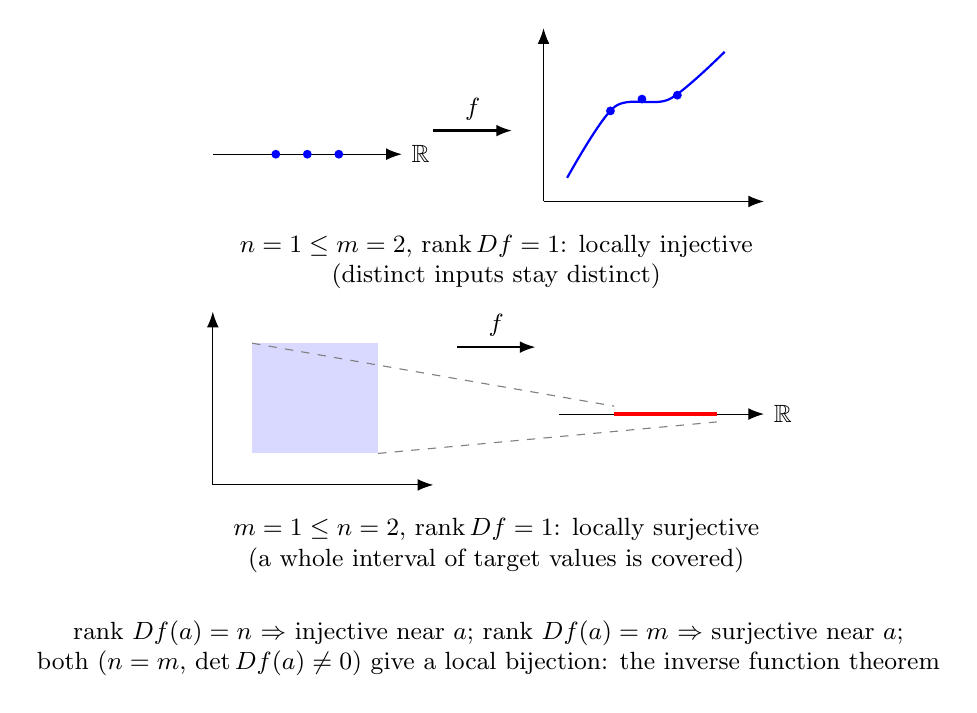
\begin{tikzpicture}[every node/.style={font=\small}, >={Latex[length=2mm]}]
	\begin{scope}
		\draw[->] (-0.2,0) -- (2.2,0) node[right, font=\small] {$\mathbb{R}$};
		\fill[blue] (0.6,0) circle (1.6pt); \fill[blue] (1.0,0) circle (1.6pt); \fill[blue] (1.4,0) circle (1.6pt);
		\draw[->, thick] (2.6,0.3) -- (3.6,0.3) node[midway, above, font=\small] {$f$};
		\draw[->] (4.0,-0.6) -- (6.8,-0.6); \draw[->] (4.0,-0.6) -- (4.0,1.6);
		\draw[blue, thick] plot[smooth] coordinates {(4.3,-0.3) (4.9,0.6) (5.6,0.7) (6.3,1.3)};
		\fill[blue] (4.85,0.55) circle (1.6pt); \fill[blue] (5.25,0.7) circle (1.6pt); \fill[blue] (5.7,0.75) circle (1.6pt);
		\node[anchor=north, align=center] at (3.4,-0.9) {$n=1\le m=2$, $\operatorname{rank}Df=1$: locally injective\\ (distinct inputs stay distinct)};
	\end{scope}
	\begin{scope}[yshift=-3.6cm]
		\draw[->] (-0.2,-0.6) -- (2.6,-0.6); \draw[->] (-0.2,-0.6) -- (-0.2,1.6);
		\fill[blue!15] (0.3,-0.2) rectangle (1.9,1.2);
		\draw[->, thick] (2.9,1.15) -- (3.9,1.15) node[midway, above, font=\small] {$f$};
		\draw[->] (4.2,0.3) -- (6.8,0.3) node[right, font=\small] {$\mathbb{R}$};
		\draw[red, very thick] (4.9,0.3) -- (6.2,0.3);
		\draw[gray, dashed] (0.3,1.2) -- (4.9,0.4);
		\draw[gray, dashed] (1.9,-0.2) -- (6.2,0.2);
		\node[anchor=north, align=center] at (3.4,-0.9) {$m=1\le n=2$, $\operatorname{rank}Df=1$: locally surjective\\ (a whole interval of target values is covered)};
	\end{scope}
	\node[anchor=north, align=center] at (3.3,-5.8) {rank $Df(a)=n$ $\Rightarrow$ injective near $a$; rank $Df(a)=m$ $\Rightarrow$ surjective near $a$;\\ both ($n=m$, $\det Df(a)\neq0$) give a local bijection: the inverse function theorem};
\end{tikzpicture}
\end{document}
